\vspace*{0.3cm}
\begin{center}
    {\huge Appendix}
\end{center}
\vspace*{0.5cm}

\setcounter{theorem}{0}
This appendix provides both theoretical and experimental materials and is organized as follows: Section~\ref{sec:supp_background} provides a more detailed background on graph neural networks. Section~\ref{sec:supp_theory} presents proofs of Theorem 1 and 2. Section~\ref{sec:supp_experiments} provides experimental details and additional results. Section~\ref{sec:supp_interpretation} provides details on the model interpretation and additional visualization results.

\section{Background on Graph Neural Networks}\label{sec:supp_background}
The overarching idea of a graph neural network is to iteratively update a node's embedding by incorporating information sent from its neighbors. \citet{xu2018how} provide a general framework of the steps incorporated in this process by generalizing the different frameworks into ,  and  steps. The various flavors of GNNs can be typically understood as variations within these three functions. For a given layer , the  step aggregates (e.g. using the sum or mean) the representations of the neighbors of a given node, which is then combined with the given node's representation from the previous layer in the  step. This is followed by a non-linear function, such as , and the updated node representations are then passed to the next layer. These two steps are repeated for as many layers as there are in the network. It is worth noting that the output of these two steps provides representations of nodes which accounts for local sub-structures of size only increased by one, which would thus require a very deep network to capture interactions between the given node and all other nodes (the depth should not be smaller than the diameter of the graph). At the end of the network, the \READOUT\ function provides a pooling function to convert the representations to the appropriate output-level granularity (e.g. node-level or graph-level). Both the  and  steps must be invariant to node permutations.  

\section{Theoretical Analysis}\label{sec:supp_theory}
\subsection{Controllability of the Representations from the Structure-Aware Attention}
\begin{theorem}
Assume that  is a Lipschitz mapping with the Lipschitz constant denoted by  and the structure extractor  is bounded by a constant  on the space of subgraphs. For any pair of nodes  and  in two graphs  and  with the same number of nodes , the distance between their representations after the structure-aware attention is bounded by:
    
    where  denotes the subgraph representation at node  for any  and  similarly, and  and  denote the multiset of subgraph representations in  and  respectively. Denoting by  the set of permutations between  and ,  is a matching metric between two multisets of representations with the same cardinality, defined as
    
     and  are constants given by:
    
\end{theorem}
\begin{proof}


    Let us denote by 
    
    and by  for any  with its -th coefficient
    
    Then, we have
    
    where  is an arbitrary permutation and we used the triangle inequality. Now we need to bound the two terms respectively. We first bound the second term:
    
    where the first inequality is a triangle inequality, the second inequality uses the Lipschitzness of . And for the first term, we can upper-bound it by
    
    where by abuse of notation,  denotes the vector whose -th entry is  for any . The first inequality comes from a simple matrix norm inequality, and the second inequality uses the fact that  function is -Lipschitz (see \eg \citet{gao2017properties}). Then, we have
    
    where the first inequality comes from , the second one uses the Cauchy-Schwarz inequality and the third one uses the definition of spectral norm and the bound of the structure extractor function. Then, we obtain the following inequality
    
    By combining the upper bounds of the first and the second term, we obtain an upper bound for the distance between the structure-aware attention representations:
    
    for any permutation , where 
    
    Finally, by taking the infimum over the set of permutations, we obtain
    the inequality in the theorem.
\end{proof}

\subsection{Expressivity Analysis}
Here, we assume that  can be any continuous mapping and it is approximated by an MLP network through the universal approximation theorem~\citep{hornik1991approximation} in practice.
\begin{theorem}
Assume that the space of node attributes  is countable. For any pair of nodes  and  in two graphs  and , assume that there exists a node  in  such that  for any  and a node  in  such that its subgraph representation  for any . Then, there exists a set of parameters and a mapping  such that their representations after the structure-aware attention are different, \ie , if their subgraph representations are different, \ie .
\end{theorem}
\begin{proof}
    This theorem amounts to showing the injectivity of the original dot-product attention with respect to the query, that is to show
    
    is injective in , where
    
    Here we consider the offset terms that were omitted in Eq.~\eqref{eq:Attention}.
    Let us prove the contrapositive of the theorem. We assume that  for any set of parameters and any mapping  and want to show that . 
    
    Without loss of generality, we assume that  and  have the same number of nodes, that is . Otherwise, one can easily add some virtual isolated nodes to the smaller graph. Now if we take , all the softmax coefficients will be identical and we have
    
    Thus, by Lemma 5 of \citet{xu2018how}, there exists a mapping  such that the multisets  and  are identical. 
    
    As a consequence, we can re-enumerate the nodes in two graphs by a sequence  (by abuse of notation, we keep using  here) such that  for any . Then, we can rewrite the equality  as
    
    Now since there exists a node  in  such that its attributes are different from all other nodes, \ie  for any , we can find a mapping  such that  is not in the span of . Then, by their independence we have
    
    for any , ,  and .
    
    On the one hand, if we take , we have for any ,  and  that
    
    On the other hand if we take  we have for any ,  and  that
    
    where the second equality is obtained by replacing  with  in the above equality. Then, we can rewrite the above equality as below:
    
    If we denote by  the feature mapping associated with the dot product kernel  and  the correspond reproducing kernel Hilbert space, we then have for any  and  that
    
    Since by assumption there exists a  such that  and  is a universal kernel~\citep{micchelli2006universal},  is dense in  and we have . We can then conclude, by the injectivity of , that
    
    for any , and thus . Now by taking  and , we obtain the theorem.
\end{proof}


\section{Experimental Details and Additional Results}\label{sec:supp_experiments}
In this section, we provide implementation details and additional experimental results.  

\subsection{Computation Details}
All experiments were performed on a shared GPU cluster equipped with GTX1080, GTX1080TI, GTX2080TI and TITAN RTX. About 20 of these GPUs were used simultaneously, and the total computational cost of this research project was about 1k GPU hours.

\subsection{Datasets Description}
We provide details of the datasets used in our experiments, including ZINC~\citep{ZINC}, CLUSTER~\citep{dwivedi2020benchmarkgnns}, PATTERN~\citep{dwivedi2020benchmarkgnns}, OGBG-PPA~\citep{hu2020open} and OGBG-CODE2~\citep{hu2020open}. For each dataset, we follow their respective training protocols and use the standard train/validation/test splits and evaluation metrics.

\paragraph{ZINC.} The ZINC dataset is a graph regression dataset comprised of molecules, where the task is to predict constrained solubility. Like \citet{dwivedi2020benchmarkgnns}, we use the subset of 12K molecules and follow their same splits.

\paragraph{PATTERN and CLUSTER.} PATTERN and CLUSTER \citet{dwivedi2020benchmarkgnns} are synthetic datasets that were created using Stochastic Block Models \citep{PatternCluster2018}. The goal for both datasets is node classification, with PATTERN focused on detecting a given pattern in the dataset, and with CLUSTER focused on identifying communities within the graphs. For PATTERN, the binary class label corresponds to whether a node is part of the predefined pattern or not; for CLUSTER, the multi-class label indicates membership in a community. We use the splits as is used in \citet{dwivedi2020benchmarkgnns}.

\paragraph{OGBG-PPA.} PPA \citep{hu2020open} is comprised of protein-protein association networks where the goal is to correctly classify the network into one of 37 classes representing the category of species the network is from. Nodes represent proteins and edges represent associations between proteins. Edge attributes represent information relative to the association, such as co-expression. We use the standard splits provided by~\citet{hu2020open}.

\paragraph{OGBG-CODE2.} CODE2 \cite{hu2020open} is a dataset containing source code from the Python programming language. It is made up of Abstract Syntax Trees where the task is to correctly classify the sub-tokens that comprise the method name. We use the standard splits provided by~\citet{hu2020open}.

\subsection{Hyperparameter Choices and Reproducibility}\label{sec:supp_hyperparameter}
\paragraph{Hyperparameter choice.}
In general, we perform a very limited hyperparameter search to produce the results in Table~\ref{tab:comparison_to_SOTA} and Table~\ref{tab:comparison_to_ogb_SOTA}. The hyperparameters for training SAT models on different datasets are summarized in Table~\ref{tab:supp_hyperparameter}, where only the dropout rate and the size of the subgraph  are tuned ( ). We use fixed RWPE~\citep{dwivedi2022graph} with SAT on ZINC, PATTERN and CLUSTER. In all experiments, we use the validation set to select the dropout rate and the size of the subtree or subgraph  . All other hyperparameters are fixed for simplicity, including setting the readout method to mean pooling. We did not use RWPE on OGBG-PPA and OGBG-CODE2 as we observed very little performance improvement. Note that we only use  for the -subgraph SAT models on CLUSTER and PATTERN due to its large memory requirement, which already leads to performance boost compared to the -subtree SAT using a larger . Reported results are the average over 4 seeds on ZINC, PATTERN and CLUSTER, as is done in~\citet{dwivedi2020benchmarkgnns}, and averaged over 10 seeds on OGBG-PPA and OGBG-CODE2.

\begin{table}[]
    \centering
    \caption{Hyperparameters for SAT models trained on different datasets. RWPE- indicates using  steps in the random walk positional encoding, which results in a -dimensional vector as the positional representation for each node.}
    \label{tab:supp_hyperparameter}
    \begin{tabular}{lccccc}
        \toprule
Hyperparameter & \textbf{ZINC} & \textbf{CLUSTER} & \textbf{PATTERN} & \textbf{OGBG-PPA} & \textbf{OGBG-CODE2} \\
         \midrule
         \#Layers & 6 & 16 & 6 & 3 & 4 \\
         Hidden dimensions & 64 & 48 & 64 & 128 & 256 \\
         FFN hidden dimensions & \multicolumn{5}{c}{Hidden dimensions} \\
         \#Attention heads & 8 & 8 & 8 & 8 &  \\
         Dropout & \multicolumn{5}{c}{} \\
         Size of subgraphs  & \multicolumn{5}{c}{} \\
         Readout method & mean & None & None & mean & mean \\
         Absolute PE & RWPE-20 & RWPE-3 & RWPE-7 & None & None \\ \midrule
         Learning rate & 0.001 & 0.0005 & 0.0003 & 0.0003 & 0.0001 \\
         Batch size & 128 & 32 & 32 & 32 & 32 \\
         \#Epochs & 2000 & 200 & 200 & 200 & 30 \\
         Warm-up steps & 5000 & 5000 & 5000 & 10 epochs & 2 epochs \\
         Weight decay & 1e-5 & 1e-4 & 1e-4 & 1e-4 & 1e-6 \\
         \bottomrule
    \end{tabular}
\end{table}

\paragraph{Optimization.}
All our models are trained with the AdamW optimizer~\citep{loshchilov2018decoupled} with a standard warm-up strategy suggested for Transformers in~\citet{vaswani2017attention}. We use either the L1 loss or the cross-entropy loss depending on whether the task is regression or classification. The learning rate scheduler proposed in the Transformer is used on the ZINC, PATTERN and CLUSTER datasets and a cosine scheduler~\citep{loshchilov2016sgdr} is used on the larger OGBG-PPA and OGBG-CODE2 datasets.

\paragraph{Number of parameters and computation time.}
In Table~\ref{tab:supp_number_parameter}, we report the number of parameters and the training time per epoch for SAT with -subtree GNN extractors using the hyperparameters selected from Table~\ref{tab:supp_hyperparameter}. Note that the number of parameters used in our SAT on OGB datasets is smaller than most of the state-of-art methods.

\begin{table}[]
    \centering
    \caption{Number of parameters and training time per epoch for -subtree SAT models using the hyperparameters in Table~\ref{tab:supp_hyperparameter}. Various GNNs are used as the base GNN in SAT.}
    \label{tab:supp_number_parameter}
    \begin{tabular}{lccccc}
        \toprule
& \textbf{ZINC} & \textbf{CLUSTER} & \textbf{PATTERN} & \textbf{OGBG-PPA} & \textbf{OGBG-CODE2} \\
         \midrule
         Base GNN & \multicolumn{5}{c}{\#Parameters} \\
         GCN & 421k & 571k & 380k & 766k & 14,030k \\
         GIN & 495k & 684k & 455k & 866k & 14,554k \\
         PNA & 523k & 741k & 493k & 1,088k & 15,734k \\ 
         \midrule
         Base GNN & \multicolumn{5}{c}{GPU time on a single TITAN RTX/epoch} \\ 
         GCN & 6s & 142s & 40s & 308s & 40min \\
         GIN & 6s & 144s & 62s & 310s & 40min \\
         PNA & 9s & 178s & 90s & 660s & 55min \\
         \bottomrule
    \end{tabular}
\end{table}

\subsection{Additional Results}
We provide additional experimental results on ZINC, OGBG-PPA and OGBG-CODE2.

\subsubsection{Additional Results on ZINC}
We report a more thorough comparison of SAT instances using different structure extractors and different readout methods in Table~\ref{tab:supp_zinc}. We find that SAT models with PNA consistently outperform other GNNs. Additionally, the readout methods have very little impact on the prediction performance.

\begin{table}
\centering
  \caption{Test MAE for SAT models using different structure extractors and readout methods on the ZINC dataset.}
  \label{tab:supp_zinc}
  \resizebox{\textwidth}{!}{
\begin{sc}
\begin{tabular}{ll|ccc|ccc}
            \toprule
& & \multicolumn{3}{c}{\textbf{w/o edge attributes}} & \multicolumn{3}{c}{\textbf{w/ edge attributes}} \\ \midrule
            & Base GNN & Mean & Sum & Cls & Mean & Sum & Cls \\ 
            \midrule
            \multirow{4}{*}{k-subtree SAT} 
            & GCN & 0.1740.009 & 0.1700.010 & 0.1679.005 & 0.1270.010 & 0.1170.008 & 0.1150.007 \\ & GIN & 0.1660.007 & 0.1620.010 & 0.1570.002 & 0.1150.005 & 0.1120.008 & 0.1040.003 \\
            & GraphSAGE & 0.1640.004 & 0.1650.008 & 0.1560.005 & - & - & - \\
            & PNA & 0.1470.001 & 0.1420.008 & \textbf{0.1350.004} & 0.1020.005 & 0.1020.003 & \textbf{0.0980.008} \\ \midrule
            \multirow{4}{*}{k-subgraph SAT} 
            & GCN & 0.1840.002 & 0.1860.007 & 0.1840.007 & 0.1140.005 & 0.1030.002 & 0.1030.008 \\ & GIN & 0.1620.013 & 0.1580.007 & 0.1620.005 & 0.0950.002 & 0.0970.002 & 0.0980.010 \\
            & GraphSAGE & 0.1680.005 & 0.1650.005 & 0.1690.005 & - & - & -\\
            & PNA & 0.1310.002 & 0.1290.003 & \textbf{0.1280.004} & 0.0940.008 & \textbf{0.0890.002} & 0.0930.009 \\
            \bottomrule
        \end{tabular}
\end{sc}
}
\end{table}

\subsubsection{Additional Results on OGBG-PPA}
Table~\ref{tab:supp_ppa} summarizes the results for -subtree SAT with different GNNs compared to state-of-the-art methods on OGBG-PPA. All the results are computed from 10 runs using different random seeds.

\begin{table}
  \centering
  \caption{Comparison of SAT and SOTA methods on the OGBG-PPA dataset. All results are computed from 10 different runs.}
  \label{tab:supp_ppa}
  \begin{sc}
        \begin{tabular}{lccc}
        \toprule
        {}& \multicolumn{2}{c}{\textbf{OGBG-PPA}} \\
        Method & Test accuracy & Validation accuracy \\
        \midrule
        GCN & 0.68390.0084 & 0.64970.0034 \\
        GCN-Virtual Node & 0.68570.0061 & 0.65110.0048	\\
        GIN & 0.68920.0100 & 0.65620.0107 \\
        GIN-Virtual Node & 0.70370.0107 & 0.66780.0105 \\
        \midrule
        Transformer & 0.64540.0033 & 0.62210.0039 \\
        \midrule
        k-subtree SAT-GCN & 0.74830.0048 & \textbf{0.70720.0030} \\
        k-subtree SAT-GIN & 0.73060.0076 & 0.69280.0058 \\
        k-subtree SAT-PNA & \textbf{0.75220.0056} & 0.70250.0064 \\
        \bottomrule
        \end{tabular}
    \end{sc}
\end{table}

\subsubsection{Additional Results on OGBG-CODE2}
Table~\ref{tab:supp_code2} summarizes the results for -subtree SAT with different GNNs compared to state-of-the-art methods on OGBG-CODE2. All the results are computed from 10 runs using different random seeds.

\begin{table}
  \caption{Comparison of SAT and SOTA methods on the OGBG-CODE2 dataset. All results are computed from 10 different runs.}
  \label{tab:supp_code2}
  \centering
  \begin{sc}
        \begin{tabular}{lccc}
        \toprule
        {}& \multicolumn{2}{c}{\textbf{OGBG-CODE2}} \\
        Method & Test F1 score & Validation F1 score \\
        \midrule
        GCN & 0.15070.0018 & 0.13990.0017 \\
        GCN-Virtual Node & 0.15810.0026 & 0.14610.0013	\\
        GIN & 0.14950.0023 & 0.13760.0016 \\
        GIN-Virtual Node & 0.15810.0026 & 0.14390.0020 \\
        \midrule
        Transformer & 0.16700.0015 &  0.15460.0018 \\
        GraphTrans & 0.18300.0024 & 0.16610.0012 \\
        \midrule
        k-subtree SAT-GCN & 0.19340.0020 & \textbf{0.17770.0011} \\
        k-subtree SAT-GIN & 0.19100.0023 & 0.17480.0016 \\
        k-subtree SAT-PNA & \textbf{0.19370.0028} & 0.17730.0023 \\
        \bottomrule
        \end{tabular}
    \end{sc}
\end{table}

\begin{comment}
\subsection{Additional Experiments on Positional Encoding}

\leo{We now provide additional experiments to showcase the role of the positional encoding, by including a comparison of when the positional encoding is random. To generate random encodings, we took the existing positional encodings of a graph and randomly permuted them (RW-perm, LAP-perm), as well as generated a random positional encoding based on white noise (Random). We show the results in the figure below. We include the results shown in the main paper (None, LAP, RW). The main paper only compares the LAP and RW positional encodings to no positional encoding (None), as ``No positional encoding" best isolates the effect of positional encoding, whereas a random positional encoding would remove the positional encoding, but also add noise to the model. 
}
\begin{figure}[htbp]
    \centering
\centering

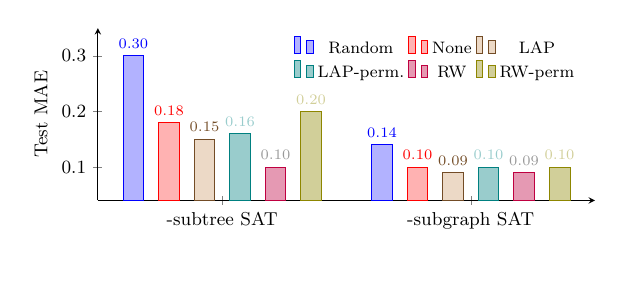
\begin{tikzpicture}[scale=0.75]
 
\begin{axis} [ybar = .25cm,
    yshift            = 5mm,
    width=10cm,
    height=4.5cm,
    bar width = 10pt,
    axis lines = left,
    xmin = 0.5, 
    xmax = 2.5,
ymax = 0.3,
    label style       = {font={\small}},
    ticklabel style={font=\small},
    ylabel={Test MAE},
    xlabel={\textcolor{white}{x}},
    enlarge y limits = {abs = .05},
    ytick = {0.10,0.20, 0.30},
    xtick = {1,2},
    xticklabels={\small -subtree SAT, \small -subgraph SAT},
    nodes near coords,
    every node near coord/.append style={font=\scriptsize},
    nodes near coords style={/pgf/number format/.cd,fixed, zerofill,precision=2},
    legend style={font=\footnotesize, legend columns=3, draw=none},
]
\addplot coordinates {(1,0.30) (2,0.14)}; \addplot coordinates {(1,0.18) (2,0.10)}; 

\addplot coordinates {(1,0.15) (2,0.09)}; \addplot[fill=teal, draw=teal, fill opacity=0.4, text=teal] coordinates {(1,0.16) (2,0.10)}; 

\addplot[fill=purple, draw=purple, fill opacity=0.4] coordinates {(1,0.10) (2,0.09)}; \addplot[fill=olive, fill opacity=0.4, text=olive, draw=olive] coordinates {(1,0.20) (2,0.10)}; 

\legend{Random, None, LAP, LAP-perm., RW, RW-perm}
\end{axis}

\end{tikzpicture}
\label{fig:pos_enc_rebuttal}
%
     \caption{A comparison of the effect of a positional encoding (RW, LAP) to no positional encoding (None), a white noise positional encoding (Random), and random permutations of the RW and LAP positional encodings (RW-perm, LAP-perm.}
    \vspace{-.7cm}
\end{figure}
\end{comment}

\newpage

\section{Model Interpretation}\label{sec:supp_interpretation}
In this section, we provide implementation details about the model visualization.

\subsection{Dataset and Training Details}
We use the Mutagenicity dataset~\citep{KKMMN2016}, consisting of 4337 molecular graphs labeled based on their mutagenic effect. We randomly split the dataset into train/val/test sets in a stratified way with a proportion of 80/10/10. We first train a two-layer vanilla Transformer model using RWPE. The hidden dimension and the number of heads are fixed to 64 and 8 respectively. The CLS pooling as described in Section~\ref{sec:pooling} is chosen as the readout method for visualization purpose. We also train a -subtree SAT using exactly the same hyperparameter setting except that \emph{it does not use any absolute positional encoding}.  is fixed to 2. For both models, we use the AdamW optimizer and the optimization strategy described in Section~\ref{sec:supp_hyperparameter}. We train enough epochs until both models converge. While the classic Transformer with RWPE achieves a test accuracy of 78\%, the -subtree SAT achieves a 82\% test accuracy.

\subsection{Additional Results}

\paragraph{Visualization of attention scores.}
Here, we provide additional visualization examples of attention scores of the [CLS] node from the Mutagenicity dataset, learned by SAT and a vanilla Transformer. Figure~\ref{fig:supp_attn_score} provides several examples of attention learned weights. SAT generally learns sparser and more informative weights even for very large graph as shown in the left panel of the middle row. 


\begin{figure}[htbp]
    \includegraphics[width=.4\textwidth]{figures/attn/colorbar_full.pdf} \\
    \begin{center}
\includegraphics[width=.48\textwidth]{figures/attn4293.pdf}
    \includegraphics[width=.48\textwidth]{figures/attn/attn1707.pdf} \\
    \includegraphics[width=.48\textwidth]{figures/attn/attn497.pdf}
    \includegraphics[width=.48\textwidth]{figures/attn/attn500.pdf} \\
    \includegraphics[width=.48\textwidth]{figures/attn/attn956.pdf}
    \includegraphics[width=.48\textwidth]{figures/attn/attn3347.pdf}
\caption{Attention visualization of SAT and the Transformer. The middle column shows the attention weights of the [CLS] node learned by our SAT model and the right column shows the attention weights learned by the classic Transformer with RWPE.}\label{fig:supp_attn_score}
\end{center}

\section{Relationship to Subgraph Neural Networks and Graph Pooling}

\leo{
In the following we clarify the relationship (and differences) of SAT to Subgraph Neural Networks  \citep{alsentzer2020subgraph} as well as to the general topic of graph pooling.

\subsection{Differences to Subgraph Neural Networks}
Subgraph Neural Networks (SNN) \cite{alsentzer2020subgraph} explores explicitly incorporating position, neighborhood and structural information, for the purpose of solving the problem of subgraph prediction. SNN generates representations at the level of subgraph (rather than node). SAT, on the other hand, is instead motivated by modeling the \emph{structural interaction} (through the dot-product attention) between nodes in the Transformer architecture by generating node representations that are structure-aware. This structure-aware aspect is achieved via a structure extractor, which can be any function that extracts local structural information for a given node and does not necessarily need to explicitly extract subgraphs. For example, the -subtree GNN extractor does not explicitly extract the subgraph, but rather only uses the node representation generated from a GNN. This aspect also makes the -subtree SAT very scalable. In contrast to SNN, the input to the resulting SAT is not subgraphs but rather the original graph, and the structure-aware node representations are computed as the query and key for the dot-product attention at each layer.  

\subsection{Relationship to Graph Pooling}
In GNNs, structural information is traditionally incorporated into node embeddings via the neighborhood aggregation process. A supplemental way to incorporate structural information is through a process called \emph{local pooling}, which is typically based on graph clustering \citep{ying2018hierarchical}. Local pooling coarsens the adjacency matrix at layer  in the network by, for example, applying a clustering algorithm to cluster nodes, and then replacing the adjacency matrix with the cluster assignment matrix, where all nodes within a cluster are connected by an edge. An alternative approach to the pooling layer is based on sampling nodes \citep{gao2019graph}. While \citet{rethinkpooling2020} found that these local pooling operations currently do not improve performance relative to more simple operations, local pooling could in theory be incorporated into the existing SAT's -subtree and -subgraph GNN extractors, as it is another layer in a GNN.
}

\begin{comment}
    "Graph pooling based on graph clustering can be used to identify structural similarity between nodes.
Understand the structural information of a graph using subgraphs or graph pooling."
\end{comment}


\end{figure}